% Set the document class and theme
\documentclass{beamer}
\usetheme{CambridgeUS}
\setbeamertemplate{caption}[numbered]
\setbeamertemplate{theorems}[numbered]
\setbeamerfont{footnote}{size=\tiny}

\usepackage{./presentation_macros}

\addbibresource{references.bib}

% Add presentation data here

% Text in the square brackets `[]' are shown in the footer. If not mentioned,
% then text in the curly braces `{}' are used as theme defaults.

\title[AKA for V2X]{Anonymous Key Agreements for V2X Communication}
\date{May 1, 2024}
\author{Gautam Singh}
\institute[IITH]{Indian Institute of Technology Hyderabad}

% Presentation begins here

\begin{document}
    \maketitle
    \tableofcontents
    \section{Introduction}
    
    \begin{frame}
        \frametitle{V2X Related Terminology}
        \begin{figure}
            \centering
            \resizebox{.8\textwidth}{!}{\begin{tikzpicture}[
    mindmap,
    concept color=red!55!black,
    text=white
]
    \node [concept] {\textbf{V2X}\\\small{Vehicle-to-Everything}}
    child[grow=150] {node[concept] {\textbf{V2D}\\\tiny{Vehicle-to-Device}}}
    child[grow=210] {node[concept] {\textbf{V2G}\\\tiny{Vehicle-to-Grid}}}
    child[grow=0] {
        node[concept] {\textbf{V2N}\\\tiny{Vehicle-to-Network}}
        child[grow=60] {node[concept] {\textbf{V2C}\\\tiny{Vehicle-to-Cloud}}}
        child[grow=120] {node[concept] {\textbf{V2P}\\\tiny{Vehicle-to-Pedestrian}}}
        child[concept color=green,grow=240,text=black] {node[concept] {\textbf{V2V}\\\tiny{Vehicle-to-Vehicle}}}
        child[concept color=green,grow=300,text=black] {node[concept] {\textbf{V2I}\\\tiny{Vehicle-to-Infrastructure}}}
    };
\end{tikzpicture}}
            \caption{A breakdown of V2X.}
        \end{figure}
    \end{frame}

    \begin{frame}
        \frametitle{Message Types in V2X}
        \begin{enumerate}
            \item<1-> \textbf{Cooperative Awareness Messages} (CAMs)
            \footcite{etsi-en-302-637} and \textbf{Basic Safety Messages} (BSMs)
            \footcite{J2735_202309V2XCommunications}.
            \begin{enumerate}
                \item Exchanged between vehicles to create awareness and support
                cooperative performance of vehicles in the road network.
                \item Includes status information such as time, position, speed,
                active systems, vehicle dimensions, etc.
                \item Broadcasted unencrypted in 5.9 GHz channel (ETSI ITS-G5).
                \item \textbf{Huge privacy concerns and threats!}
            \end{enumerate}
            \item<2-> Other types of messages
            \begin{enumerate}
                \item \textbf{Signal Phase and Timing} (SPaT)
                \item \textbf{Roadside Infrastructure Information} (MAP)
            \end{enumerate} 
        \end{enumerate}
    \end{frame}

    \begin{frame}
        \frametitle{Motivation and Goals}
        \begin{enumerate}
            \item<1-> Do we \emph{really} need to encrypt CAMs?
            \begin{itemize}
                \item Google (Maps) may already be profiling us!
                \item Focus on encrypting more sensitive messages and
                information sent less frequently.
            \end{itemize}
            \item<2-> Unlimited privacy.
            \item<3-> Better security guarantees (privacy, authenticity,
            confidentiality).
        \end{enumerate}
    \end{frame}

    \section{Preliminaries}

    \begin{frame}
        \frametitle{Pairings}
        \begin{definition}{Pairing\footcite{GraduateCourseApplied}}
            Let \(\bG_0 = \abrak{g_0}\), \(\bG_1 = \abrak{g_1}\), \(\bG_T\) be
            three cyclic groups of prime order \(q\). A \emph{pairing} is an
            efficiently computable function \(e: \bG_0 \times \bG_1 \rightarrow
            \bG_T\) satisfying the following properties:
            \begin{enumerate}
                \item \emph{bilinear}: for all \(u, u^{\prime} \in \bG_0\) and
                \(v, v^{\prime} \in \bG_1\), we have
                \begin{align}
                    e\brak{uu^{\prime}, v} &= e\brak{u,v}e\brak{u^{\prime},v} \\
                    e\brak{u, vv^{\prime}} &= e\brak{u,v}e\brak{u, v^{\prime}}
                \end{align}
                \item \emph{non-degenerate}: \(g_T := e\brak{g_0, g_1}\) is a
                generator of \(\bG_T\).
            \end{enumerate}
        \end{definition}
        \begin{enumerate}
            \item<2-> Here, \(\bG_0\) and \(\bG_1\) are called \emph{source
            groups} and \(\bG_T\) is called the \emph{target group}.
            \item<3-> When \(\bG_0 = \bG_1\), the pairing is said to be
            \emph{symmetric}.
        \end{enumerate}
    \end{frame}

    \begin{frame}
        \frametitle{Anonymous Key Agreement}
        \begin{enumerate}
            \item<1-> A key agreement protocol where two parties agree on a
            shared secret key, without being able to determine the other party.
            \item<2-> Pairing-based anonymous key agreement for V2X.
            \item<3-> We use a pairing-based anonymous key agreement involving a
            private key generator
            (PKG)\footcite{katePairingBasedOnionRouting2007}.
            \begin{enumerate}
                \item PKG has its own master private and public key.
                \item PKG uses master secret key to generate secret keys for
                clients.
                \item Clients use this secret key to establish the shared secret
                key.
            \end{enumerate}
            \item<4-> Clients can now create \textbf{psuedonyms} or fake
            identities \(id \rightarrow \brak{\cH\brak{id}}^r,
            \cH:\mathcal{ID}\rightarrow\cG, r \in \bZ_q\).
        \end{enumerate}
    \end{frame}

    \begin{frame}
        \frametitle{Attributes, Credentials, Anonymous Credentials}
        \begin{enumerate}
            \item<1-> \textbf{Attributes}: Labels associated with a user that
            describe them fully, such as role of a user.
            \item<2-> \textbf{Credential}: Data possessed by a user that
            demonstrates their attributes.
            \item<3-> \textbf{Anonymous Credential}: Data possessed by a user
            that demonstrates their attributes, \emph{without revealing any
            additional information} about their identity.
            \item<4-> For V2X
            \begin{itemize}
                \item Anonymous credentials issued to vehicles regularly.
                \item We use DGSA (Digital Group Signatures with Attributes)
                \footcite{camenischZoneEncryptionAnonymous2020}, which gives us
                a \textbf{randomizable} group element as the credential \(\sigma
                \rightarrow \sigma^r, r \in \bZ_q\).
            \end{itemize}
        \end{enumerate}
    \end{frame}

    \section{Our Proposition}
    \begin{frame}
        \frametitle{Proposed Message Flow Diagram}
        \begin{figure}
            \centering
            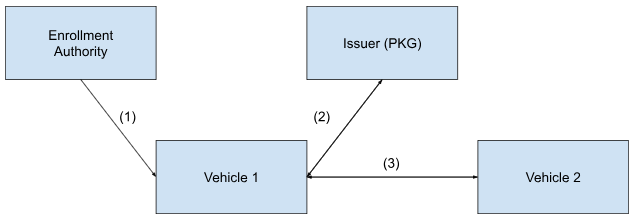
\includegraphics[width=\columnwidth]{figs/flow.png}
            \caption{Message flow of the proposed scheme.}
            \label{fig:new-flow}
        \end{figure}
    \end{frame}

    \begin{frame}
        \frametitle{Proposed Message Flow}
        \begin{enumerate}
            \item<1-> Enrollment authority issues certificate to vehicle.
            \begin{itemize}
                \item Certificate is a long-term credential that can be used to
                revoke the holder in case of misbehaviour.
            \end{itemize}
            \item<2-> Issuer issues DGSA credentials and secret key after
            verifying certificate.
            \begin{itemize}
                \item This secret key is different from secret key associated
                with certificate.
                \item DGSA credentials guarantee authenticity.
                \item Anonymous key agreement ensures that user identities
                remain anonymous throughout communication.
                \item This is done periodically every \emph{epoch}.
            \end{itemize}
            \item<3-> Vehicles exchange DGSA-signed randomized psuedonyms to
            generate shared key for futher communicaton.
            \begin{itemize}
                \item Used in verifying legitimacy of the other party.
            \end{itemize}
        \end{enumerate}
    \end{frame}

    \begin{frame}
        \frametitle{Analysis}
        \begin{enumerate}
            \item<1-> \textbf{Advantages}
            \begin{itemize}
                \item Fully anonymous communication, unlimited privacy between
                communicating parties.
                \item Third parties cannot identify who is communicating.
                \item Useful for sending extremely sensitive data.
                \item Malicious vehicles can be revoked.
            \end{itemize}
            \item<2-> \textbf{Disadvantages}
            \begin{itemize}
                \item Lots of pairing computations, for DGSA and for anonymous
                key agreement. Incurs computational overheads.
                \item Works for single-hop connections only.
                \item May not be scalable to communicating with many vehicles
                simultaneously in terms of storage overhead.
            \end{itemize}
        \end{enumerate}
    \end{frame}

    \section{Conclusion}
    \begin{frame}
        \frametitle{Future Work}
        \begin{enumerate}
            \item<1-> Encrypt V2X messages like CAMs.
            \item<2-> Improve efficiency of the present work.
            \begin{itemize}
                \item Use one of DGSA or anonymous key agreement, but not both?
            \end{itemize}
            \item<3-> A new workflow for encryption using zones
            \footcite{camenischZoneEncryptionAnonymous2020} and zone managers
            \footcite{yuePracticalPrivacypreservingCommunication2022b}
        \end{enumerate}
    \end{frame}

\end{document}
